\cite{FP}
% ==================================================
%	Aufbau
% ==================================================

\section{Aufbau}
\begin{figure}
\centering 
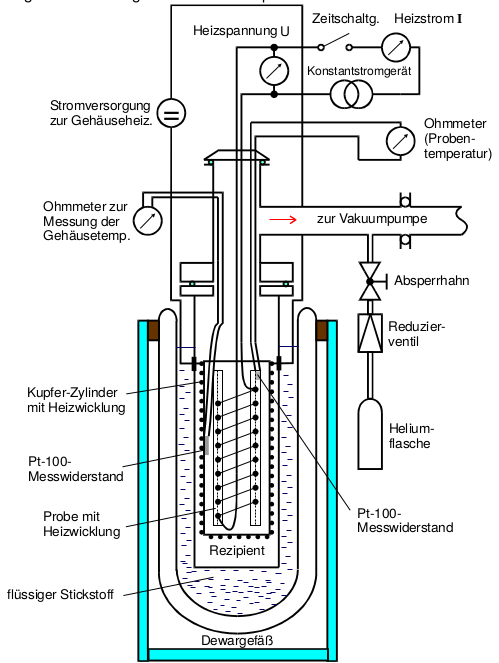
\includegraphics[scale=1]{figures/setup.pdf}
\caption{Schematische Abbildung des Versuchsaufbaus. \cite{FP}}
\label{fig:aufbau:setup}
\end{figure}
Der Versuchsaufbau ist in Abbildung \ref{fig:aufbau:setup} zu sehen. Der 
Rezipient befindet sich in einem Gehäuse, das mittels einer Vakuumpumpe 
evakuiert werden kann. Über ein Ventil kann das Gehäuse mit Helium befüllt 
werden. Rezipient und Gehäuse besitzen jeweils eine eigene Heizwicklung, sodass 
diese über getrennte Stromversorgungen einzeln geheizt werden können. Die 
Temperaturmessung geschieht mittels Widerstandsmessung eines Pt-100-Messwiderstandes, 
für den die Beziehung 
\begin{equation}
T = 0.00135 R^2 + 2.296 R -243.02
\end{equation}
zwischen dem gemessenen Widerstandswert $R$ in $\Omega$ und der Temperatur $T$ in 
$\si{\celsius}$ gilt. Das Gehäuse befindet sich in einem Dewargefäß.